\section{Anforderung an die technische Lösung}
Im nachfolgendem Abschnitt wird auf die Verordnung über das Fast-Track Verfahren und die Anforderungen nach dem digitale Gesundheitsanwendungen bewertet und als Erstattungsfähig eingestuft werden, beleuchtet. Diese wird mithilfe eines zugrundeliegenden DiGA-Fast-Track-Canvas
% des "Platform Ecosystem Manager - Healthcare (PEMH) 
(Quelle: Knape2020) veranschaulicht.
\subsection{ Bewertungsgrundlage einer DiGA }
Die Digitale Gesundheitsanwenungen-Verordnung (DIGVA) vom 8. April 2020, gilt als Richtlinie und Bewertungsgrundlage des Fast-Track-Verfahrens. Das BfArM richtet sich ausschließlich nach diesen Vorgaben. Diese Verordnung ist für jeden einsehbar und somit eine hervorragende Grundlage für die Hersteller zur Vorbereitung auf den Antrag.
Die Verordnung gliedert sich in 9 Abschnitte, die schriftlich festlegen was eine DiGA\footnote{Digitale Gesundheitsanwendung} auszeichnet.
\begin{enumerate}
	\item \small{Antragsberechtigung und Antragsinhalte}
	\item \small{Anforderungen an Sicherheit, Funktionstauglichkeit, Datenschutz und Sicherheit sowie Qualität digitaler Gesundheitsanwendungen}
	\item \small{Anforderungen an den Nachweis positiver Versorgungseffekte}
	\item \small{Ergänzende Vorschriften für das Verwaltungsverfahren}
	\item \small{Inhalte und Veröffentlichung des Verzeichnisses für digitale Gesundheitsanwendungen nach § 139e Absatz 1 des Fünften Buches Sozialgesetzbuch}
	\item \small{Beratung durch das Bundesinstitut für Arzneimittel und Medizinprodukte}
	\item \small{Gebühren und Auslagen}
	\item \small{Schiedsverfahren}
	\item \small{Schlussbestimmungen}
\end{enumerate}

Jedoch ist sie in der Form des Bundesgesetzblattes verfasst, sodass sie nicht unbedingt leserfreundlich und für jeden auf Anhieb verständlich ist. Dafür stellt das BfArm\footnote{Bundesinstitut für Arzneimittel und Medizinprodukte\label{ftn:bfarm}} online einen Leitpfaden zur Verfügung. Dieser enthält alle Informationen rund um das Themas DiGA. Von Antragsstellung bis hin zur Aufnahme ins Verzeichnis. Dieser Leitfaden des Bundesinstitut für Arzneimittel und Medizinprodukte enthält sehr viele Informationen und ist mit seinen 141 Seiten nicht gerade übersichtlich und kompakt.

Wie wäre es deshalb einen übersichtlichen Canvas zu haben, der in einer überschaubaren Form Überblick über alle relevanten Anforderungen gibt? Genau das bietet der DiGA-Fast-Track-Canvas (Quelle: Knape2020).
%des "Platform Ecosystem Manager - Healthcare (PEMH) \cite{bibid} 
Hier würden bereits alle wichtigen Punkte der Verordnung in einer kompakten Form zusammen gefasst.
Der Canvas besteht ebenfalls aus neun Haupteilen und eine Kopfbereich, der Bezeichnung der DiGA, Medizinprodukt-Risikoklasse (nach MDR), Autor, Datum und Versionsnummer zusammenfasst. Die weiteren Bereiche befassen sich mit den tieferen Grundanforderungen des Verfahrens und dienen als äquivalent zu den Abschnitten in der Verordnung. Die Überschriften sind überwiegend als Fragestellungen formuliert, sodass schnell klar ist was hier ``gefragt'' ist.
%\renewcommand{\labelenumi}{\roman{enumi})}
\begin{enumerate}
	\item \textbf{Wie lautet die medizinische Zweckbestimmung Indikation? Kontradiktion? Patientengruppe?}
	\\In diesem Abschnitt legt der Hersteller die medizinischen Zweckbestimmungen da, die laut DIGAV §2 Absatz 2 nach medizinprodukterechtlichen Vorschriften gelten. Unter anderem soll hier auch auf die ``Patientengruppen eingegangen werden, für die positive Versorgungseffekte nach den §§ 8 und 9 nachgewiesen wurde oder, im Falle der vorläufigen Aufnahme, in dem Erprobungszeitraum nachgewiesen werden sollen.'' \cite{Verordnung}
	\item \textbf{Was unterstützt die digitale Anwendung?}
	\\In diesen Abschnitt geht es darum festzustellen ob die digitale Gesundheitsanwendung zur Erkennung, Behandlung, Überwachung, Linderung, Kompensierung einer Krankheit oder Behinderung dient. Oder ob es sich hierbei um Präventionsmaßnahmen handelt. Den würde die digitale Gesundheitsanwendung nur zur Primärprävention dienen, handelt es sich hier nicht um eine DiGA und würde im Antragsfall abgelehnt werden.
	\item \textbf{Wer sind die Nutzer der digitalen Anwendung?}
	\\Hier wird Primär, wie die Fragestellung eindeutig vorgibt aus das Nutzersegment eingegangen. Denn abzuklären ist, ob Es sich bei den Nutzer nur um Patienten oder auch um Ärzte und Therapeuten gemeinsam handelt oder nur um Leistungserbringer handelt. Denn im letzteren Fall würde es sich wieder nicht um eine DiGA handeln.
	\item \textbf{Worin besteht die digitale Hauptfunktionalität der Anwendung?}
	\\Die Hauptfunktionalität ist insofern wichtig, dass es sich bei auf eine digitale Technologie beruhen sollte. Sollte dies nicht der Fall sein kann diese Anwendung ebenfalls nicht in das DiGA Verzeichnis aufgenommen werden und würde bei der Antragsstellung keine Zustimmung bekommen.
	\item \textbf{Welche DiGA-Anforderungen erfüllt der Hersteller?}
	\\Als nächstes wird auf die DiGA-Anforderungen eingegangen, die den Hersteller der digitalen Gesundheitsanwendung betreffen. Dieser Anforderungen bezieht sich vor allem auf den Abschnitt 2 im DIGAV, der sich Anforderung an die Sicherheit, Funktionstauglichkeit,Datenschutz und -sicherheit sowie Qualität vorgibt. Hier wird im §7 die notwendige Nachweis durch Zertifikate benannt und in §9 die Darlegung positiver Versorgungseffekte erklärt. Sollte einer der Ökonomischen Nutzen in der Reduzierung von Kosten liegen, würde auch dieser Antrag von der BfArm eine Abgelehnung erhalten.
	\item \textbf{Welche DiGA-Anforderung erfüllt die digitale Anwendung?}
	\\Dieser Abschnitt bietet einen guten Überblick über die Grundfunktionen, die die digitale Gesundheitsanwendung grundsätzlich erfüllen sollte. Anforderungen an die Anwendung spiegelt dich im Verlauf der gesamten Verordnung in verschiedenster Form wieder und sollte deshalb direkt vor Antragsstellung durchweg mit "ja" beantwortet sein. 
	\item \textbf{Welches sind die nächsten Schritte des Herstellers?}
	\\ Hier entsteht nach erfolgreicher Beantwortung des Canvas ein Leitfaden, welches noch Notwendige Schritte vor der Einleitung des Antrages sind und sichert somit die Hersteller ab, nichts relevantes aus den Augen zu verlieren.
	\item \textbf{Gebühren und Auslagen für Hersteller}
	\\Dieser Bereich stützt sich auf den Abschnitt 7 der Verordnung und gibt einen Ausblick auf welche Kosten in welcher Form und Höhe während des Prozess zur Einstufung als erstattungsfähigen digitale Gesundheitsanwendung anfallen.
	\item \textbf{Marktzugang}
	\\Dieser Bereich bezieht sich auf weitere Informationen, die Anwendung Typisieren . Zum Beispiel unter welchen ICD-10-Code diese Anwendung fällt.
	
\end{enumerate}

Nach Bearbeitung dieses Canvas erhält man ein gutes Verständnis über die aktuellen Situation der eigenen digitalen Anwendung und welche Schritte noch nötig sind eine erstattungsfähige Anwendung zu werden. 
\begin{figure}[H]
	\centering
	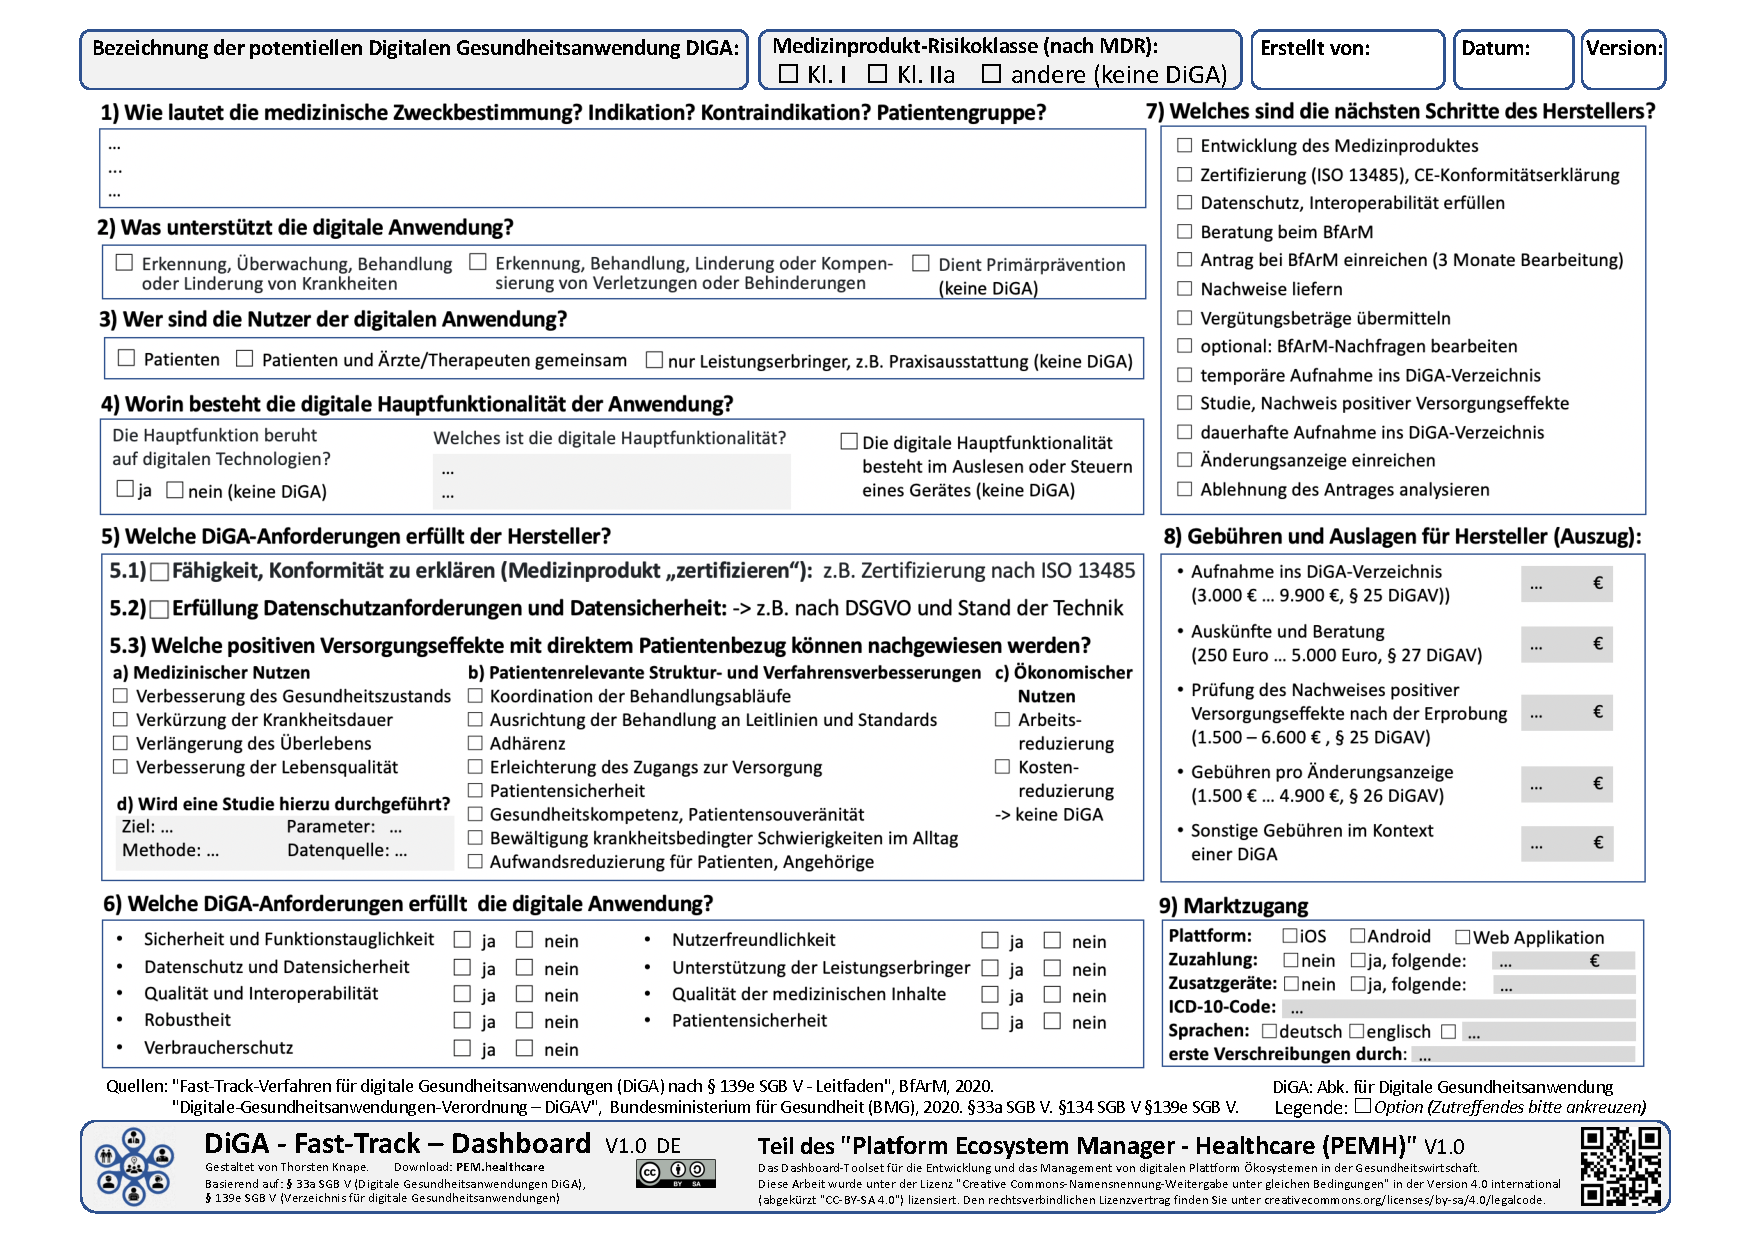
\includegraphics[width=450px, keepaspectratio]{assets/DiGA_Canvas.pdf}
	\caption[DiGA-Fast-Track-Canvas]{DiGA-Fast-Track-Canvas,~Quelle: Knape2020}
\end{figure}

Da die Anforderung an das Self-Service ist genau diese Klarheit zu schaffen, wird dieser Canvas als Grundlage für die Entwicklung des Tools dienen.

\subsection{Funktionale Anforderung des Self-Service}
Hauptfunktionalität des Self-Service wird es sein, eine Nutzeroberfläche für Hersteller anzubieten, in der Sie Angaben zu ihrer digitalen Gesundheitsanwendung machen.
Nach erfolgreichen befüllen werden die Antworten ausgewertet und einen Leitfaden über die nächsten Schritte ausgegeben. Die von dem Hersteller angegebenen Daten werden zusammen mit dem Leitfaden in einem Canvas zusammengefasst und können anschließend als PDF runter geladen werden.
\begin{figure}[H]
	\centering
	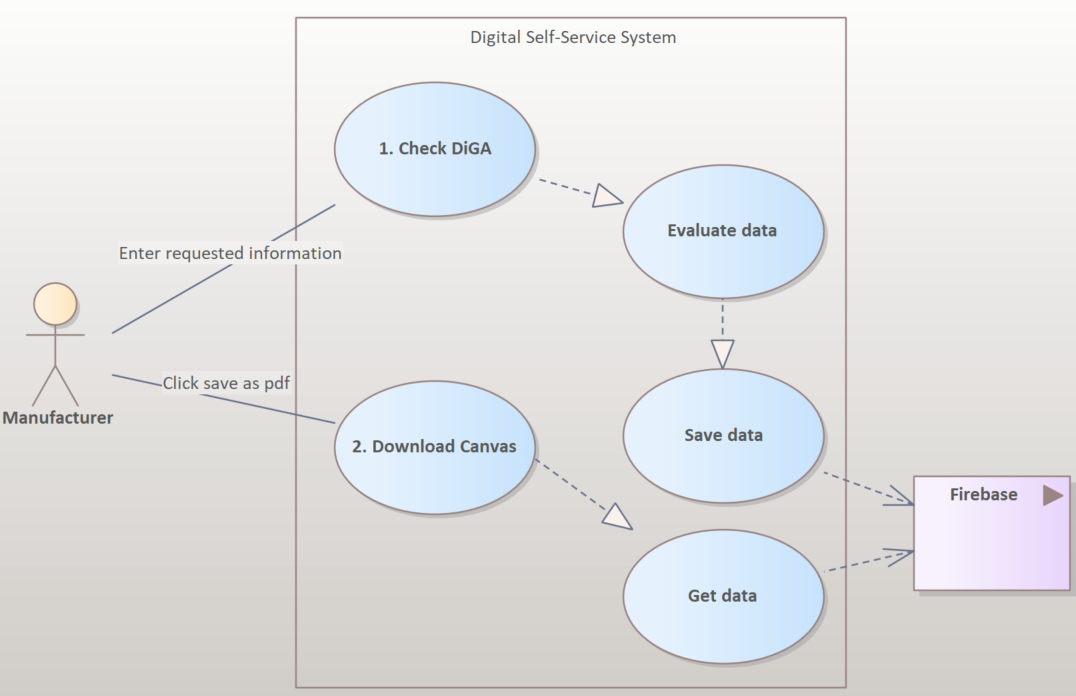
\includegraphics[width=450px, keepaspectratio]{assets/usecase1.png}
	\caption[Self-Service - Usecase Diagramm]{Self-Service - Usecase Diagramm,\\Quelle: Eigene Darstellung, Tool: \cite{enterpriseArchitect}}
\end{figure}
